\documentclass{beamer}
\mode<presentation> {

% The Beamer class comes with a number of default slide themes
% which change the colors and layouts of slides. Below this is a list
% of all the themes, uncomment each in turn to see what they look like.

\usetheme{default}
%\usetheme{AnnArbor}
%\usetheme{Antibes}
%\usetheme{Bergen}
%\usetheme{Berkeley}
%\usetheme{Berlin}
%\usetheme{Boadilla}
%\usetheme{CambridgeUS}
%\usetheme{Copenhagen}
%\usetheme{Darmstadt}
%\usetheme{Dresden}
%\usetheme{Frankfurt}
%\usetheme{Goettingen}
%\usetheme{Hannover}
%\usetheme{Ilmenau}
%\usetheme{JuanLesPins}
%\usetheme{Luebeck}
%\usetheme{Madrid}
%\usetheme{Malmoe}
%\usetheme{Marburg}
%\usetheme{Montpellier}
%\usetheme{PaloAlto}
%\usetheme{Pittsburgh}
%\usetheme{Rochester}
%\usetheme{Singapore}
%\usetheme{Szeged}
%\usetheme{Warsaw}

% As well as themes, the Beamer class has a number of color themes
% for any slide theme. Uncomment each of these in turn to see how it
% changes the colors of your current slide theme.

%\usecolortheme{albatross}
%\usecolortheme{beaver}
%\usecolortheme{beetle}
%\usecolortheme{crane}
%\usecolortheme{dolphin}
\usecolortheme{dove}
%\usecolortheme{fly}
%\usecolortheme{lily}
% \usecolortheme{orchid}
%\usecolortheme{magenta}
%\usecolortheme{seagull}
%\usecolortheme{seahorse}
%\usecolortheme{whale}
%\usecolortheme{wolverine}

%\setbeamertemplate{footline} % To remove the footer line in all slides uncomment this line
%\setbeamertemplate{footline}[page number] % To replace the footer line in all slides with a simple slide count uncomment this line

%\setbeamertemplate{navigation symbols}{} % To remove the navigation symbols from the bottom of all slides uncomment this line
}

\usepackage[T1]{fontenc}  % access \textquotedbl
\usepackage{graphicx} % Allows including images
\usepackage{booktabs} % Allows the use of \toprule, \midrule and \bottomrule in tables
\usepackage{tikz}
\def\Check{\tikz\fill[color=green, scale=0.4] (0, 0.35) -- (0.25, 0) -- (1, 0.7) -- (0.25, 0.15) -- cycle;}
\def\shortside{0.15}
\def\longside{0.25}
\def\Cross{\tikz\fill[color=red,rotate=45,scale=0.4](0,0) -- (\longside,0) -- (\longside,\longside)
-- (\longside+\shortside,\longside) -- (\longside+\shortside,0) -- (2*\longside+\shortside,0)
-- (2*\longside+\shortside,-\shortside)-- (\longside+\shortside,-\shortside)
-- (\longside+\shortside,-\shortside-\longside) --  (\longside,-\shortside-\longside)
--(\longside,-\shortside) -- (0,-\shortside) -- cycle;}

\def\dsign{$\$$}
\newcommand\comm[1]{\\ \vspace{0.2cm}\hspace{0.5cm} \footnotesize{\color{blue}\dsign #1}}
\newcommand\subitem[1]{\\ \vspace{0.2cm}\hspace{0.5cm} #1}
\def\dhyphen{\texttt{-{}-}} % double hypen
%\def\qmark{\textquotedbl} %double qoutation mark

%	TITLE PAGE

\title[Short title]{An Introduction to Git Talk} % The short title appears at the bottom of every slide, the full title is only on the title page

\author{Ehsan Zandi} % Your name
\institute[DTIT] % Your institution as it will appear on the bottom of every slide, may be shorthand to save space
{
Deutsche Telekom IT \\ % Your institution for the title page
\medskip
ehsan.zandi@telekom.de
}
\date{23.08.2021} % Date, can be changed to a custom date
%\date{\today} % Date, can be changed to a custom date

\begin{document}

\begin{frame}
\titlepage % Print the title page as the first slide
\end{frame}

\begin{frame}
\frametitle{Overview} % Table of contents slide, comment this block out to remove it
\tableofcontents % Throughout your presentation, if you choose to use \section{} and \subsection{} commands, these will automatically be printed on this slide as an overview of your presentation
\end{frame}

%	PRESENTATION SLIDES

\section{Git vs SVN} \begin{frame}{Git vs SVN}
\begin{itemize}
  \item Git is a fully distributed version control system (VCS)
  \item Each user (PC/Laptop) is an exact clone of the remote repository
    \begin{itemize}
      \item Each user is a repository (log, revert, merge, branch, etc)
      \item No network connection required, except to sync with central repo (pull/push/fetch)
      \item merge and rebasing can be done offline
    \end{itemize}
  \item Git is much faster than SVN
  \item Git's repositories are much smaller than SVN
  \item Git's branches are much simpler and less resource heavy than SVN
  \item Git is much better in branch auditing and merge handling
  \item As many backups as the number of users
  \item Content integrity using SHA-1 hash
  \end{itemize}
\end{frame}

\begin{frame}{Git vs SVN}
  \begin{figure}
    \begin{center}
    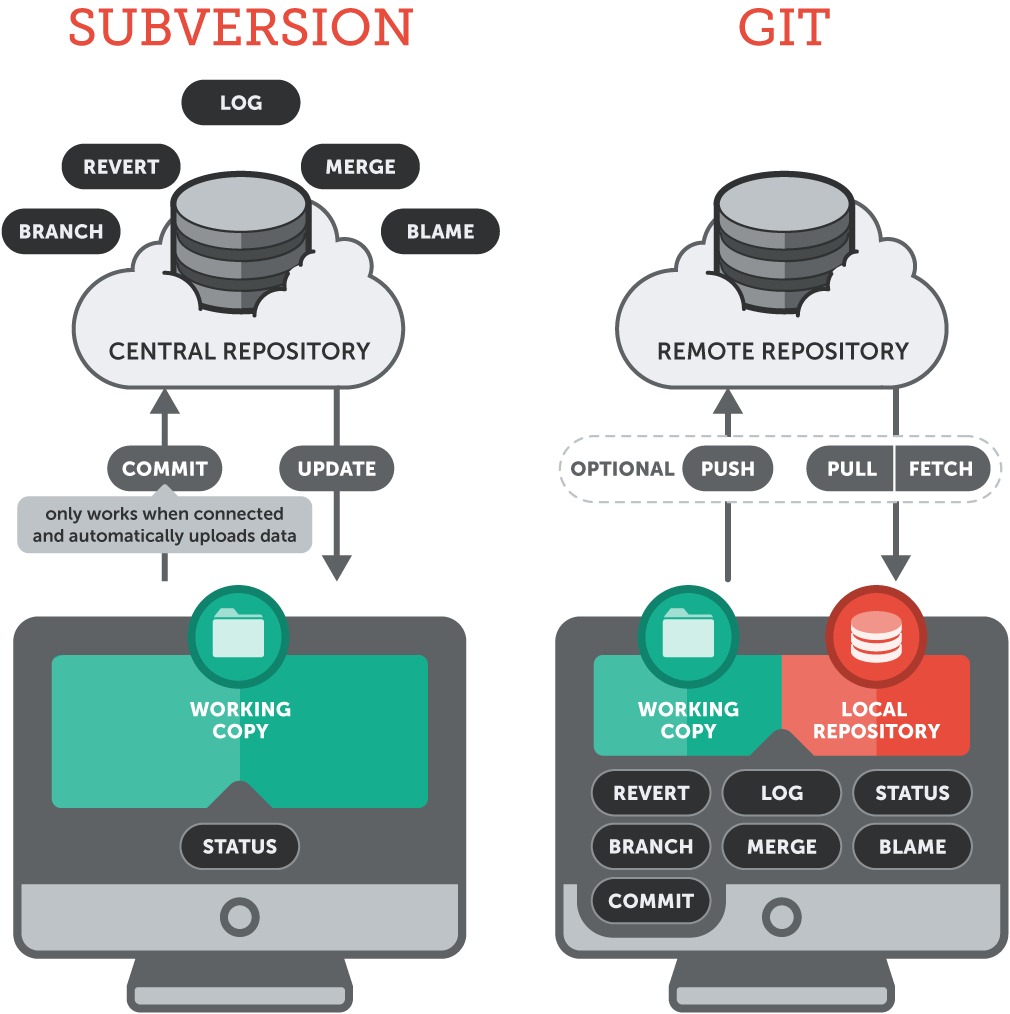
\includegraphics[width=0.5\linewidth]{pics/git-vs-svn.png}
    \vspace{-0.3cm}
    \caption{\footnotesize Centralized vs distributed VCS (Source: www.git-tower.com)}
  \end{center}
\end{figure}
\end{frame}

\begin{frame}{Git vs SVN}
  \begin{center}
  \begin{tabular}{ c || c | c  }
         & SVN & Git \\ \hline\hline
    \textbf{License} & Open-source (Apache) & GNU \\
    \textbf{Distributed-ness} & Centralized & Fully Distributed  \\
    \textbf{Speed} & \Cross & \Check \\
    \textbf{Storage} & \Cross & \Check \\
    \textbf{Integrity Guarantee} & \Cross & \Check \\
    \textbf{Brnaching \& merging} & \Cross & \Check \\
    \textbf{Stashing} & \Cross & \Check \\

      \end{tabular}
    \end{center}
\end{frame}



\section{Git Basics}
\begin{frame}{Git Basics}{Architecture}
  \begin{itemize}
    \item Remote: The central repo (on a host machine/server, e.g., Github or Gitlab)
      {\color{red}$\rightarrow$ is identified by the alias "origin"}
    \item Repository: The local repo (.git sub-directory inside your working directory), created by "git init" or "git clone", i.e., ceartion/clonining
    \item Index or staging area: State between the working directory and repository (after modifying and before commiting)
    \item Workspace or working directory: your local machine, including all directories, sub-directories, and files of your project
  \end{itemize}
  \begin{figure}
    \begin{center}
    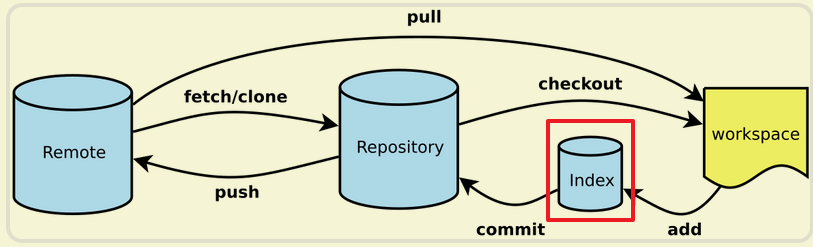
\includegraphics[width=0.8\linewidth]{pics/architecture.png}
    \vspace{-0.3cm}
    \caption{\footnotesize Git architecture (Source: www.stackoverflow.com)}
  \end{center}
\end{figure}

\end{frame}

\begin{frame}{Git Basics}{Definitions}
  \begin{itemize}
    \item \textbf{origin}: A shorthand name for the remote repo
      \comm{git remote show} (shows "origin" as output)
      \comm{git remote show origin} (shows detailed info on origin)
\item \textbf{branch}: A movable pointer to a commit
\item \textbf{master (or sometimes main)}: Default name of the (first) branch: can be changed
\item \textbf{HEAD}: A special pointer that tells on (the tip of) which branch you are.
\item \textbf{origin/HEAD}: A special pointer that tells on which branch the remote repo is.
\end{itemize}
\end{frame}



\begin{frame}{Git Basics}{Add/Commit}
  \begin{itemize}
    \item \textbf{git add}: To add a new file or modified into the staging (index) area. It makes 
      the changes ready for commiting.
      \comm{git add FILE\_NAME}
      \comm{git add .} (adds all the changes current directory and sub-directories)
    \item \textbf{git commit}: To put the staged files into the (local) repo. Such changes can be tracked, i.e.,
      revert, log, etc.
      \comm{git commit -m "A proper message"}
  \end{itemize}
  \begin{figure}
    \begin{center}
    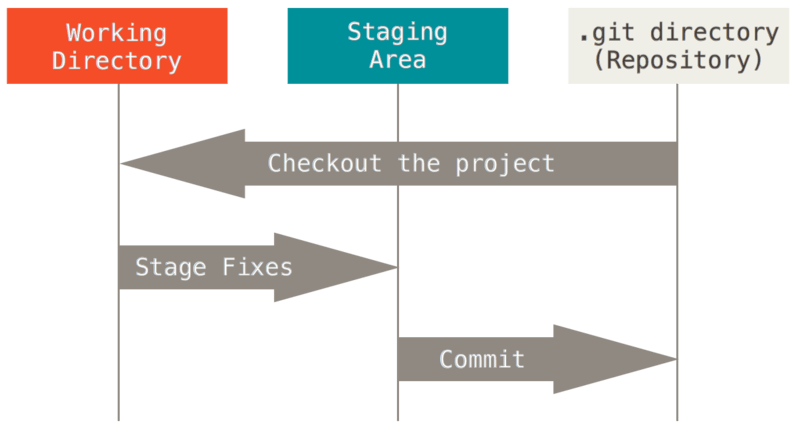
\includegraphics[width=0.55\linewidth]{pics/areas.png}
    \vspace{-0.3cm}
    \caption{\footnotesize Git areas (Source: https://git-scm.com)}
  \end{center}
\end{figure}
\end{frame}

\begin{frame}{Git Basics}{Initializing a repo}
  \begin{itemize}
    \item Creating a local repo (without any remote)
    \comm{git init} (creates .git sub-directory)
    \comm{echo "hello world." $>>$ firstFile.txt} (makes changes in  working area)
    \comm{git status} (You see that your commit has some hash value)
    \comm{git add firstFile.txt} (puts your changes into staging area)
    \comm{git status} (You see that your commit has some hash value)
    \comm{git commit -m "A proper message"} (Now you have your first commit on the default branch master)
    \begin{itemize}
      \item Hint:
      {\tiny {\color{blue}git commit -am "A proper message"} (combines "git add" and "git commit")}
    \end{itemize}
    \comm{git status} (A clean repo and one commit with a hash value)
    \comm{git branch -m master main} (renames the branch master to main)
    \comm{git remote} (Output is empty since there is no remote repo)
  \end{itemize}
\end{frame}



\begin{frame}{Git Basics}{Status and Log}
\begin{itemize}
\item Status and log
\comm{git status} (Shows the status of the repo)
\comm{git log} (Shows the commit log on the current branch)
\comm{git log SOME\_BRNACH} (Shows the commit log on a specific branch)
\comm{git log \dhyphen all} (Shows the commit log on all branches)
\comm{git log -p} (Shows the commit log and the content difference of files per commit, combines 
git log and git diff)
\comm{git log \dhyphen decorate \dhyphen oneline \dhyphen graph \dhyphen all} (Very useful graph-like history)
\end{itemize}
\end{frame}
\begin{frame}{Git Basics}{Aliases}
\begin{itemize}
\item Git Aliases, some useful examples:
\comm{git config \dhyphen global alias.g \sq log \dhyphen decorate \dhyphen oneline \dhyphen graph \dhyphen all\sq} (makes "git g" an alias for the previous long command)
\comm{git config \dhyphen global alias.l log} (makes "git l" an alias for "git log")
\comm{git config \dhyphen global alias.loa \sq log \dhyphen oneline \dhyphen all\sq} (makes "git loa" an alias
for "git log \dhyphen oneline \dhyphen all")
\comm{git config \dhyphen global alias.s status} (makes "git s" an alias for "git status")
\comm{git config \dhyphen global alias.b status} (makes "git b" an alias for "git branch")
\comm{git config \dhyphen global alias.ch checkout} (makes "git ch" an alias for "git checkout")

\end{itemize}
\end{frame}

\begin{frame}{Git Basics}{Difference}
\begin{itemize}
\item Comparing files on the same branch
\comm{git diff} (shows the difference between working and staging area for all files\rightarrow to be staged, i.e., git add)
\comm{git diff SOME\_FILE} (shows the difference between working and staging area for a given file)
\comm{git \dhyphen staged diff} (shows the difference between staging area and last commit for all files\rightarrow to be commited)
\comm{git \dhyphen cached diff} (the same as above)
\comm{git diff HEAD} (combines "git diff" and "git diff \dhyphenr staged")
\item Comparing files between two branches
  \comm{git branch BRANCH\_A..BRANCH\_B} (compares all files)
  \comm{git branch BRANCH\_A..BRANCH\_B SOME\_FILE} (compares only a given files)
\end{itemize}
\end{frame}

\begin{frame}{Git Basics}{Checkout}
\begin{itemize}
\item Go back to some specific commit
\comm{git checkout 53c5105} (8 first digits out of a 40-long hexadecimal digit HASH-1)
\begin{itemize}
\item Hint: Now you get the message {\color{red} HEAD detachhed at 53c5105}
  \comm{git checkout master} (to reattach the HEAD to master)
  \comm{git switch master} (to reattach the HEAD to master)
  \comm{git switch -} (to reattach the HEAD to last branch)
\end{itemize}
  \comm{git checkout 53c5105 SOME\_FILE} (checks out only the given files to the given commit)
  \comm{git checkout .} (checks out everything to last commit)
  \comm{git checkout HEAD .} (the same as above)
  \comm{git checkout \dhyphen  FILE\_NAME} (restore the file to the last commit)
\end{itemize}
\end{frame}

\section{Stash Area} \begin{frame}{Hidden Area}{Stash}
  {\footnotesize Switching between branches or checking out older commits, while having unclean staging area, 
  are avoided or cause conflicts. Staged (but not commited) changes can hidden into the stash area to clean the  working area. Then, you can do whatever 
you want, while changes in the stash remians, until they are applied or deleted.}
\begin{itemize}
\item 
  \comm{git stash}  (stashes all staged changes)
  \comm{git stash save "Something"}  (stashes the changes with a label)
  \comm{git stash list} (shows the stash area, might be more than one entry)
  \comm{git stash apply stash@\{1\}} (applies the stash before most recent)
  \comm{git stash show stash@\{1\} -p} (shows content of $2^{\text{nd}}$ newest stash)
  \comm{git stash apply} (applies the most recent stash)
  \comm{git stash pop} (applies and then deletesi the stash)
  \comm{git stash clear} (clears the stash area)
  \comm{git stash drop stash@\{2\}} (deletes the $3^\text{rd}$ newest stash)
\end{itemize}
\end{frame}

\section{Branches}  \begin{frame}{Branches in Git}{Creating, Displaying, and Switching}
  \begin{itemize}
\item Creating a branch
  \comm{git branch NEW\_BRANCH} (creates a new branch)
  \comm{git checkout -b BRANCH\_NAME} (creates and switch)
  \comm{git switch -c BRANCH\_NAME} (creates and switch, from Git 2.23)
\item Displaying branches
  \comm{git branch} (shows only local branches)
  \comm{git branch -r} (shows only remote branches)
  \comm{git branch -a} (shows all branches)
\item Switching between branches
  \comm{git checkout BRANCH\_NAME} (switches to another branch)
  \comm{git switch BRANCH\_NAME} (switches to another branch)
\end{itemize}
\end{frame}

 \begin{frame}{Branches in Git}{Comparing, Merging, Renaming, and Deleting}
  \begin{itemize}
\item Comparing two branches
  \comm{git branch BRANCH\_A..BRANCH\_B} (compares all files)
  \comm{git branch BRANCH\_A..BRANCH\_B SOME\_FILE} (compares only a given files)
\item Merging branches
  \comm{git merge BRANCH\_B} (merges branch b into branch a, you should be in branch a)
\item Renaming a branch
  \comm{git branch -m OLD\_NAME NEW\_NAME} 
\item Deleting a branch 
  \comm{git branch -d BRANCH\_FOR\_DELETION} (deletes a branch)
\end{itemize}
\end{frame}

\begin{frame}{Remote Branches}{Creating and Deleting}
  \begin{itemize}
\item Creating remotes branch in command line, where branch A already exists locally
\comm{git checkout -b origing/BRANCH\_A}
\item Deleting a remote branch 
  \comm{git push -d origin/BRANCH\_FOR\_DELETION} 
\end{itemize}
\end{frame}

\section{Remote Repositories} \begin{frame}{Git Basics}{Cloning}
  \begin{itemize}
  \item Getting a remote repo:
    \comm{git init}
    \comm{git remote add origin REPO\_ADDRESS/REPO\_NAME.git}
    \comm{git pull origin master}
    \comm{git branch \dhyphen set-upstream-to=origin/master}
  \end{itemize}
  \begin{itemize}
  \item or the easy way $\rightarrow$ git clone
    \comm{git clone REPO\_ADDRESS/REPO\_NAME.git}
    \comm{git clone /home/ehszandi/Public/gitIntro.git} (This is an example)
  \end{itemize}
  Now the repository is cloned and you can work on it!
\end{frame}

\section{Undoing Changes} \begin{frame}{Undoing Changes}{Checkout}
\begin{itemize}
\item Go back to some specific commit
\comm{git checkout 53c5105} (8 first digits out of a 40-long hexadecimal digit HASH-1)
\begin{itemize}
\item Hint: Now you get the message {\color{red} HEAD detachhed at 53c5105}
  \comm{git checkout master} (to reattach the HEAD to master)
  \comm{git switch master} (to reattach the HEAD to master)
  \comm{git switch -} (to reattach the HEAD to last branch)
\end{itemize}
  \comm{git checkout 53c5105 SOME\_FILE} (checks out only the given files to the given commit)
  \comm{git checkout .} (checks out everything to last commit)
  \comm{git checkout HEAD .} (the same as above)
  \comm{git checkout -- FILE\_NAME} (restore the file to the last commit)
\end{itemize}
\end{frame}

\begin{frame}{Undoing Changes}{Restore}
\begin{itemize}
  \item Unmodify changes (to the last commit)
    \comm{git restore FILE\_NAME}
  \item Restore one file to three commits prior to HEAD
    \comm{git restore source=HEAD~3 FILE\_NAME}
    \comm{git restore FILE\_NAME}
    \comm{git restore --staged FILE\_NAME} (unstage the file)
\end{itemize}
\end{frame}

%\begin{frame}{Undoing Changes}{Reset}
%\begin{itemize}
%
%\end{itemize}
%\end{frame}

\section{Reflog}\begin{frame}{Git Reflog}{reflog}
\begin{itemize}
    \item  Reference logs, or "reflogs", record when the tips of branches and other references were updated in the 
      \textbf{local} repository. 
    \item It expires by default after 90 days (default can be changed) 
    \item HEAD@\{0\} means the very first reflog, while HEAD@\{1\} means the second and so forth.
    \item What comes inside @\{~\} is called \textbf{qualifier}, i.e., entry number or time
    \comm{git reflog show} (shows .git/logs/HEAD in reverse order)
    \comm{git reflog show HEAD@\{0\}} (the same as above as, up to the latest reflog, i.e., HEAD@\{0\})
    \comm{git reflog show HEAD@\{2\}} (does not show the first two reflogs)
    \comm{git reflog show HEAD@\{27.Aug.2021\}} (reflogs up to the given date)
    \comm{git reflog show HEAD@\{one.week.ago\}} (reflogs up to last week)
    \comm{git reflog show master@\{one.week.ago\}} (reflogs up to last week, but only for master branch
    or any other branch)
\end{itemize}
\end{frame}

\begin{frame}{Git Reflog}{reflog}
\begin{itemize}
  \item {\color{red} Hint:} While HEAD$\sim$2 means 2 commit ago, HEAD\{2\} does not mean that. If you switch
    to another branch, it is inserted in reflog.
   \comm{git checkout HEAD$\sim$2} (checks out the 2 commits before the tip of the current branch)
    \comm{git checkout HEAD@\{2\}} (it could a commit on another branch, or even it could the same commit
   as HEAD, but only refereing to switching between branches)
\end{itemize}
\end{frame}

\begin{frame}{Git Reflog}{reflog}
\begin{itemize}
  \item {\color{red} Saving the mistakes or undoing the past:} Find the hash number of the
    state to which you want to go back using "git reflog show", then do
    one the followings:
    \comm{git reset \dhyphen hard 34a523fc} 
    \comm{git reset \dhyphen hard master@{3}} 
    \comm{git reset \dhyphen hard HEAD@{4}} 
  \item {\color{red} \Large \textbf{Limitation:}} git reflogs are \textbf{only} local
\end{itemize}
\end{frame}

\section{Rebase}\begin{frame}{Rebase}{Rebase}
\begin{itemize}
\item Rebase has two usage:
\begin{enumerate}
\item Using rebase as alternative to merge, which also cleans simplifies/cleans
the log graph. The workflow is the same as "git merge", but instead with "git rebase" command.
  \begin{figure}
    \begin{center}
    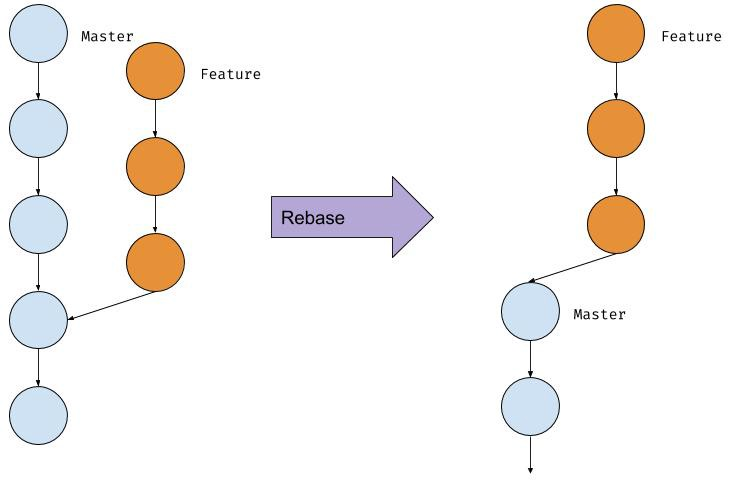
\includegraphics[width=0.4\linewidth]{pics/rebase-merge.jpeg}
    \vspace{-0.3cm}
    \caption{\footnotesize Regular architecture (Source: https://itnext.io)}
  \end{center}
\end{figure}
\item Interactive rebase to modify/delete commits
\comm{git rebase -i HEAD$\sim$3} (It starts editing the last 3 commits)
\end{enumerate}
\end{itemize}
\end{frame}

\begin{frame}{Rebase}{Rebase vs merge}
  \begin{figure}
    \begin{center}
    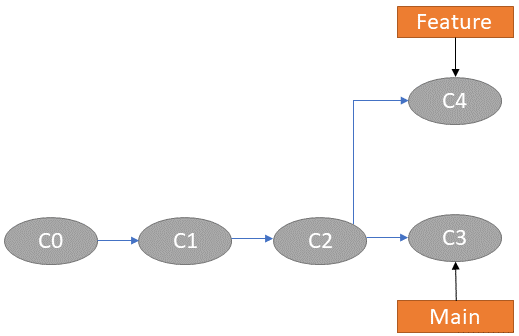
\includegraphics[width=0.6\linewidth]{pics/rebase-vs-merge-1.png}
    \vspace{-0.3cm}
  \end{center}
\end{figure}
\end{frame}

\begin{frame}{Rebase}{Rebase vs merge}
   \comm{git switch main}
   \comm{git merge merge}
  \begin{figure}
    \begin{center}
    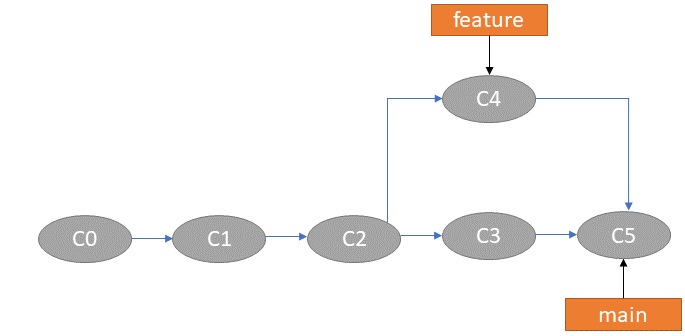
\includegraphics[width=0.6\linewidth]{pics/rebase-vs-merge-2.png}
    \vspace{-0.3cm}
  \end{center}
\end{figure}
\end{frame}

\begin{frame}{Rebase}{Rebase vs merge}
   \comm{git switch feature}
   \comm{git rebase main}
  \begin{figure}
    \begin{center}
    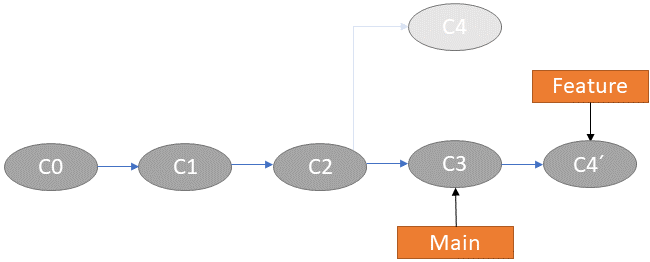
\includegraphics[width=0.6\linewidth]{pics/rebase-vs-merge-3.png}
    \vspace{-0.3cm}
  \end{center}
\end{figure}
\end{frame}

\begin{frame}{Rebase}{Rebase vs merge}

   \comm{git switch main}
   \comm{git merge feature}
%     \vspace{-3cm}
  \begin{figure}
    \begin{center}
    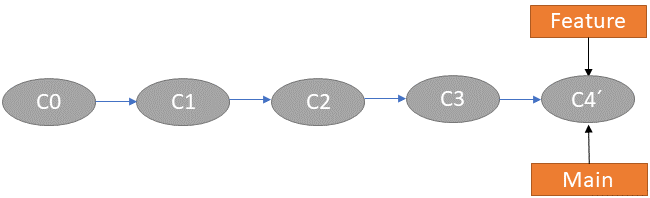
\includegraphics[width=0.6\linewidth]{pics/rebase-vs-merge-4.png}
  \end{center}
\end{figure}
\end{frame}

\section{Tag}\begin{frame}{Tag}{Create}
\begin{itemize}
  \item Tags are to refer to (important) moments of time
  \item They are used, e.g., as reference to release versions
\item There two types of tags
\begin{enumerate}
  \item \textbf{Lightweight} tag which is just a pointer to a specific commit.
    \comm{git tag -a TAG} (lightweight tag the current commit)
    \comm{git tag -a TAG HASH} (lightweight tag the given hash)
  \item \textbf{Annotated} tag which is checksummed, contains the tagger name, email, and date; have a tagging message; and can be signed and verified with GNU Privacy Guard (GPG).
    \comm{git tag -a TAG} (annotated tag the current commit)
    \comm{git tag -a TAG HASH} (annotated tag the given hash)
\end{enumerate}
\end{itemize}
\end{frame}

\begin{frame}{Tag}{List, Move, Delete, Push}
\begin{itemize}
\item Tags can be used as argument to other git commands,
  such as \emph{diff}, \emph{checkout}
    \comm{git tag} (shows all existing tags)
    \comm{git tag -l "v17*"} (shows all tags starting with v17)
    \comm{git tag -f TAG} (forces move existing tag to the current commit)
    \comm{git tag -d TAG} (deletes the tag)
  \item Git does not push the tag by default to the remote. You should tell
    git to do so, using
    \comm{git push \dhyphen tag}
\end{itemize}
\end{frame}

\section{Git Objects}\begin{frame}{Git Objects}
Each Git object has its own hash value and is
stored in .git/objects/FOLDER/FILE,
where FOLDER is the first two digit of its hash value
and the FILE Is the rest of its 38 digits. Git has 4 types of objects
\begin{enumerate}
\item\textbf{commit}: is created upon each commiting and contains a tree object, parent, author, commiter
and a message.
\item \textbf{tree}: is similar to directory in UNIX and is indeed staging area (index) and contains 
blobs and sub-trees. 
\item \textbf{blob} (binary large object): is the file content without
file name. 
\item\textbf{tag} (annotated)
\end{enumerate}
\end{frame}

\begin{frame}{Git Objects}
  \begin{figure}
    \begin{center}
    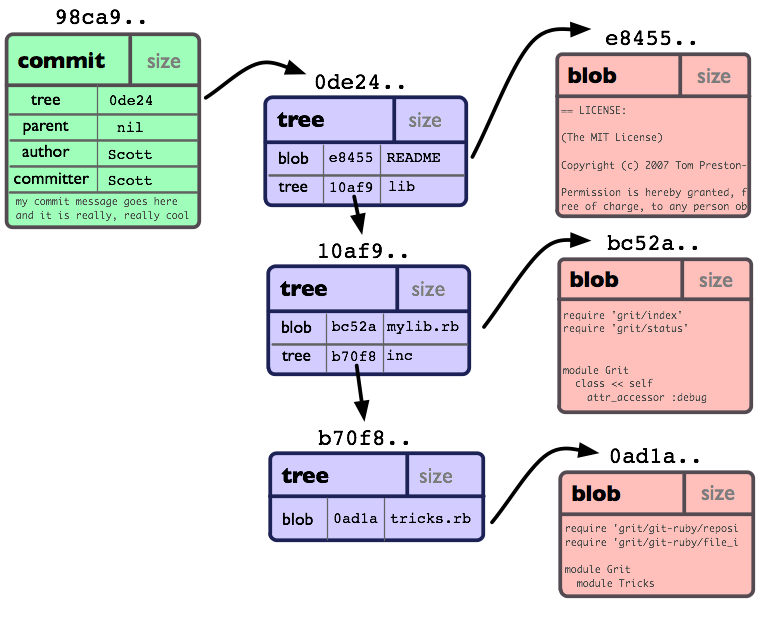
\includegraphics[width=0.8\linewidth]{pics/objects.png}
    \vspace{-0.3cm}
    \caption{\footnotesize Commit, tree and blob objects (Source: https://shafiul.github.io)}
  \end{center}
\end{figure}
\end{frame}

\begin{frame}{Git Objects}
  \begin{itemize}
      \item Create hash object
        \comm{git hash-object -w FILE} (-w stands for write. If given, saves the hash .git/objects. If not given only shows the hash)
        \comm{echo "hello" | git hash-object \dhyphen stdin -w} (created hash from standard input)
      \comm{git cat-file -t HASH} (shows the type of hash value)
      \comm{git cat-file -p HASH} (shows the content of hash value)
      \comm{git cat-file -p BRANCH\textasciicircum\{tree\}} (shows the content of tree, i.e., blobs and sub-trees, of the tip of the given branch)
      \comm{git cat-file -p HASH\textasciicircum\{tree\}} (shows the content of tree, i.e., blobs and sub-trees, of the tip of the given hash)
  \end{itemize}
\end{frame}
\begin{frame}{Git Objects}{Add, Commit in low level Git}
      This examples shows how to create, add and commit changes into
      git, without using "git add" and "git commit" commands.   
      \begin{itemize}
    \item We add one line, i.e., "hello", to the FILE (any given file) and commit it.

          \comm{echo "hello" >> FILE} (adds "hello" to the end FILE)
          \comm{git hash-object FILE -w} (outputs a hash which is used below, i.e., HASH)
      \comm{git update-index \dhyphen add \dhyphen cacheinfo 100644 HASH FILE} (adds the changes to FILE to a new staging area)
      \comm{git write-tree} (writes the staging area out to a tree object and creates a tree object with a TREE-HASH)
          \comm{git commit-tree -p PARENT-HASH -m "MESSAGE" TREE-HASH} (does what git commit -m "MESSAGE" does)
  \end{itemize}
\end{frame}


\section{Git SVN}\begin{frame}{Git SVN}{Cloning}
  \begin{itemize}
    \item \textbf{One time import from svn}:
    \comm{git svn clone -T trunk -b branches -t tags -s -A authors.txt -r14542:HEAD https://10.32.93.102:9880/svn/pegaplan}
    \item See all local and remote (svn) branches
    \comm{git branch -a}
    \item  Checkout a remote (svn) branch, e.g., 9.0, into a corresponding local branch, e.g., 9.0
  \comm{git checkout -b 9.0 remotes/origin/9.0}
  \item Check if the local branch is tracking the remote branch
  \comm{git svn dcommit -n} (-n does not actually commit, it is for dry-run)
  \item After updating the local repository, push it into the remote branch
  \comm{git svn dcommit --username="ehszandi"}
  \end{itemize}
\end{frame}

\begin{frame}{Git SVN}{Cooperation in Branches}
  \begin{itemize}
    \item If the branch is already created, only check it out (see above), otherwise
    \item Create a remote branch for debug/cooperation with colleagues and switch to the local corresponding branch
\comm{git ch -b NEW\_BRANCH remotes/origin/NEW\_BRANCH}
  \item After updating the local repository, push it into the remote branch
  \comm{git svn dcommit --username="ehszandi"}
\item Deleting a remote branch 
  \comm{git branch -d --remotes origin/BRANCH\_FOR\_DELETION} 
  \end{itemize}
\end{frame}


\section{To be learned}\begin{frame}{To be learnt}
\comm{git update-ref}
  \comm{git rev-parse BRANCH|TAG|HEAD} (gives the proper hash of it)
  \comm{it config rerere.enabled true} ("reuse recorded resolution" tells Git to remember how you’ve resolved a hunk conflict so that the next time it sees the same conflict, Git can resolve it for you automatically.)
\end{frame}


\end{document}
